%! Mode:: "TeX:UTF-8"
%! TEX program = xelatex
\PassOptionsToPackage{quiet}{xeCJK}
\documentclass[withoutpreface,bwprint]{cumcmthesis}
\usepackage{etoolbox}
\usepackage{ctex}
\BeforeBeginEnvironment{tabular}{\zihao{-5}}
\usepackage[numbers,sort&compress]{natbib}  % 文献管理宏包
\usepackage[framemethod=TikZ]{mdframed}  % 框架宏包
\usepackage{url}  % 网页链接宏包
\usepackage{subcaption}  % 子图宏包
\newcolumntype{C}{>{\centering\arraybackslash}X}
\newcolumntype{R}{>{\raggedleft\arraybackslash}X}
\newcolumntype{L}{>{\raggedright\arraybackslash}X}\renewcommand{\textbf}[1]{{\song\bfseries #1}}

\usepackage{tikz}
\usetikzlibrary{shapes.geometric, arrows.meta, positioning}

\tikzstyle{startstop} = [rectangle, rounded corners, minimum width=3cm, minimum height=1cm,text centered, draw=black, fill=red!20]
\tikzstyle{process} = [rectangle, minimum width=3.5cm, minimum height=1cm, text centered, draw=black, fill=blue!20]
\tikzstyle{decision} = [diamond, aspect=2, minimum width=3.5cm, minimum height=1cm, text centered, draw=black, fill=green!20]
\tikzstyle{arrow} = [thick,->,>=stealth]

%% 队伍编号和赛道表格（对应官方 Word 模板首页表格，置于第一页顶部、论文标题上方）
%% 填写处：MCB260XXXX 改为实际队伍编号，（A/B）改为实际赛道
\makeatletter
\let\mcm@orig@makeothertitle\makeothertitle
\renewcommand{\makeothertitle}{%
  \if@mcm@preface
    \mcm@orig@makeothertitle
  \else
    \begin{center}
      \renewcommand{\arraystretch}{1.5}
      \begin{tabular}{|>{\centering\arraybackslash}p{3.9cm}|>{\centering\arraybackslash}p{3.9cm}|}
        \hline
        队伍编号 & MCB260XXXX \\
        \hline
        赛道 & （A/B） \\
        \hline
      \end{tabular}
    \end{center}
    \vskip2ex
    \mcm@orig@makeothertitle
  \fi
}
\makeatother






















\title{基于集成学习的洪水概率预测}  % 论文标题



%%%%%%%%%%%%%%%%%%%%%%%%%%%%%%%%%%%%%%%%%%%%%%%%%%%%%%%%%%%%%
%% 正文

% 独立预览保留总论文的章节序号；正式合并时只引入章节文件。
\BeforeBeginEnvironment{tabularx}{\zihao{-5}}
\setlength{\emergencystretch}{2em}
\begin{document}
\setcounter{section}{6}
\setcounter{equation}{7}
\setcounter{figure}{1}
\setcounter{table}{5}
% 第三问正文；从总论文主文件所在目录编译，图片位于 figures/q3/。
\section{问题三的模型的建立和求解}
\label{sec:q3}

\subsection{问题分析}
问题三需要回答泥石流何时触发、能够提前多久预警，以及触发后前缘何时到达吉隆口岸、沿程推进多远。前两问已建立环境因素与源区风险之间的联系，本问在此基础上引入天气预报，先估计未来触发时刻及其区间，再通过沟道传播模型求取到达时间与距离，并评价触发区间的覆盖情况。

未来热力、水分条件及其持续时间影响风险演化，沿程速度则影响触发后的传播时间。本文以GEFS集合均值构建确定性基线，通过天气和参数扰动生成1000个情景，将不确定性依次传递至风险序列、触发时刻和分段传播过程。选取2026年同一事件的五次滚动起报回放，比较不同提前量下的触发区间与预警等级。

\subsection{模型建立}
\subsubsection{模型输入与时间基准}
模型沿用第二问的源区气象、水分状态与静态易发性结果，预报输入采用GEFS集合均值和离散度。五次起报分别为2026年8月19日、21日、23日、24日和25日00 UTC，对应名义提前量168、120、72、48和24 h；预报原生步长为6 h，覆盖起报后0至174 h。历史背景采用2021—2024年同期资料，2025年不参与标定。主要数据与参数见表\ref{tab:q3-data}。

下文时间统一采用北京时间，五次起报均为08:00。源区启动以8月26日10:52:21.9的第一阶段脱离时刻为准，口岸前缘候选参照时刻为10:59:48。题面的10:30为约记时间，本文用核实启动时刻计算误差与实际提前量，后者列于结果表中。

\begin{table}[htbp]
  \centering
  \zihao{-5}
  \caption{第三问主要数据与参数设置}
  \label{tab:q3-data}
  \begin{tabularx}{\textwidth}{p{3.2cm}X}
    \toprule
    数据或参数 & 使用方式或取值 \\
    \midrule
    GEFS集合均值、离散度 & 2 m气温、向下短波辐射、6 h累计降水及表层土壤水分；原生步长6 h \\
    历史背景与空间条件 & 2021—2024年同期10:00、事件日期前后15日背景；源区静态易发性百分位的第90百分位热点值 \\
    主模型前期窗口 & ETI融水72 h、累计降水72 h、根区水分均值120 h、前期降水15日 \\
    集合情景与持续条件 & 1000个合成相关情景；天气扰动AR(1)系数0.70；持续长度12 h \\
    ETI参数抽样范围 & 温度因子0.02—0.10；短波因子0.0047—0.0141；温度阈值0—1.5 $^\circ$C；反照率误差标准差0.03 \\
    独立降雨核验 & IMERG Late Run V07；按14 h名义延迟截断，窗口完整度至少95\% \\
    \bottomrule
  \end{tabularx}
\end{table}

源区海拔约4991 m，预报温度由起报订正值叠加GEFS相对变化得到：
\begin{equation}
 \mu_{T,\mathrm{src}}(t)=T_{\mathrm{src}}(t_i)
       +\left[\mu_{T,\mathrm{GEFS}}(t)-\mu_{T,\mathrm{GEFS}}(t_i)\right].
 \label{eq:q3-anchor}
\end{equation}
其中，$t_i$为起报时刻，$T_{\mathrm{src}}(t_i)$为源区订正温度，$\mu_{T,\mathrm{GEFS}}$为GEFS温度集合均值。根区水分也以起报状态为初值，叠加GEFS表层水分的预报变化作近似；VPD与位温梯度用于诊断起报背景。滚动指标按逐小时序列计算，降水分配保持原6 h累计量不变。


\subsubsection{双机制联合风险模型}
沿用第二问的增强温度指数模型，以气温和短波辐射表征热力作用。气温超过阈值后，温度项与吸收短波辐射项共同计入逐小时融水代理量：
\begin{equation}
 m_t=\begin{cases}
 f_T(T_t-T_0)+f_R(1-\alpha_t)\max(I_t,0), & T_t>T_0,\\
 0, & T_t\leq T_0.
 \end{cases}
 \label{eq:q3-eti}
\end{equation}
其中，$T_t$为源区温度，$T_0$为温度阈值，$\alpha_t$为反照率，$I_t$为向下短波辐射；$m_t$单位为mm/h，$f_T$单位为mm/(h\,$^\circ$C)，$f_R$单位为mm/[h\,(W/m$^2$)]。确定性基线取$f_T=0.05$、$f_R=0.0094$、$T_0=1\,{}^\circ$C；集合模型按表\ref{tab:q3-data}中的范围分别均匀抽样。

为比较不同量纲的触发因素，将72 h融水累计量、72 h降水量、15日前期降水和120 h根区水分均值转换为各自历史分布中的百分位，分别记为$H_t$、$R_t$、$P_t$和$U_t$。其中，15日前期降水通过与历史CHIRPS背景的尺度匹配计算。前期降水与根区水分共同描述湿润背景，取二者中位数为$A_t$；短时降水与湿润背景的几何平均构成降雨—水分分支，再与热力分支组合，得到
\begin{equation}
 \begin{aligned}
 A_t&=\operatorname{median}(P_t,U_t), &
 W_t&=\sqrt{R_tA_t},\\
 D_t&=1-(1-H_t)(1-W_t), &
 J_t&=\sqrt{S D_t}.
 \end{aligned}
 \label{eq:q3-risk}
\end{equation}
式中，$H_t$、$W_t$分别为热力—冰冻圈分支与降雨—水分分支，$D_t$为综合动态评分。降水量小或湿润背景偏低时，几何平均会抑制$W_t$；任一分支升高均可提高$D_t$。空间项$S$取源区AOI内静态易发性百分位的第90百分位，减小单个极端像元的影响，最终得到源区相对风险指数$J_t\in[0,1]$。

\subsubsection{集合情景与不确定性传播}
固定融水参数，将GEFS集合均值代入式\eqref{eq:q3-risk}，得到确定性基线风险序列。在此基础上，按天气预报离散度、ETI参数范围和反照率误差构造1000个合成情景，逐一计算风险与触发时刻。

天气扰动需同时保留相邻时次的连续性与变量间的相关性。为此，在6 h原生步长上采用AR(1)过程，以相关矩阵$\boldsymbol C$描述温度、辐射、降水和土壤水分的联合扰动：
\begin{equation}
 \begin{aligned}
 \boldsymbol z_{n,k}&=\rho\boldsymbol z_{n,k-1}
       +\sqrt{1-\rho^2}\,\boldsymbol\varepsilon_{n,k},
       \quad\boldsymbol\varepsilon_{n,k}\sim N(\boldsymbol0,\boldsymbol C),\\
 \boldsymbol C&=\begin{pmatrix}
 1&0.50&-0.25&-0.20\\
 0.50&1&-0.35&-0.10\\
 -0.25&-0.35&1&0.20\\
 -0.20&-0.10&0.20&1
 \end{pmatrix},\qquad \rho=0.70.
 \end{aligned}
 \label{eq:q3-ar}
\end{equation}
其中，$n$为情景编号，$k$为6 h时次，矩阵变量依次为温度、短波辐射、降水和土壤水分。$\rho=0.70$控制扰动在相邻时次的延续程度，$\boldsymbol C$控制同一时次的变量联系，二者均作为固定情景参数。

温度、短波和降水的扰动尺度，由GEFS离散度与第二问GFS分时效核查的平均绝对误差按平方和开根合并。两段3 h降水误差按同一规则转换为6 h尺度，120 h以外沿用75—120 h误差档。GFS误差进入离散度项，预报均值仍由GEFS确定。反照率叠加标准差0.03的情景误差，并截断至0.05—0.95；每个情景内的ETI参数保持不变。

\subsubsection{触发时间区间与预警规则}
预警时间用于识别持续高风险的开始，触发时间则用于定位该过程中的危险峰值。以历史联合风险的第80百分位$q_{0.80}$为关注阈值，连续12个小时格点达到阈值时，将该段过程的起点记为预测关注起点；起报时已满足条件的，记为即刻关注。

在此基础上，以12 h尾随平均风险衡量前期条件的持续累积，取其最大值对应窗口的结束时刻作为触发时刻。对第$n$个情景，定义
\begin{equation}
 B_n(t)=\frac{1}{12}\sum_{r=0}^{11}J_n(t-r\,\mathrm{h}),
 \qquad
 \widehat t_n=\underset{t\in\mathcal T_i}{\arg\max}\, B_n(t).
 \label{eq:q3-trigger}
\end{equation}
其中，$\mathcal T_i$为评价窗内完整12 h窗口的结束时刻集合；峰值并列时取最早者。最高平均风险达到$q_{0.80}$的情景记为支持触发，并保留其触发时刻。触发时刻取累积窗口的结束时刻，关注起点则按逐小时持续越阈规则确定。

回放评价窗从起报开始，止于核实启动后24 h与可用预报末时刻中的较早者。支持比例为1000个情景中满足触发条件的情景占比，用于描述所设情景下的触发支持程度。对有效触发时刻排序，取中位数为点估计，取2.5\%和97.5\%分位数为区间端点，构成有触发支持条件下的95\%情景区间。

区间两端各扩展3 h，将6 h原生步长的影响计入操作区间：
\begin{equation}
 \mathcal I_{\mathrm{raw}}=[Q_{0.025}(\widehat t),Q_{0.975}(\widehat t)],
 \quad
 \mathcal I_{\mathrm{op}}=[Q_{0.025}(\widehat t)-3\,\mathrm{h},
                         Q_{0.975}(\widehat t)+3\,\mathrm{h}].
 \label{eq:q3-interval}
\end{equation}
其中，$Q_p(\widehat t)$为有效触发时刻的第$p$分位数。原始区间反映情景差异，操作区间在此基础上计入半个原生时间步长。

预警等级以$J_t$的集合中位数划分。连续12 h达到历史$q_{0.80}$、$q_{0.90}$、$q_{0.95}$和$q_{0.99}$时，依次进入蓝、黄、橙、红色，对应阈值为0.7803、0.8464、0.8905、0.9486。该等级反映历史相对风险位置；取相邻两次起报最高持续等级中的较低者，进一步考察滚动预报的一致性。

\subsubsection{分段传播模型}
将源区至口岸的路径划分为A—B、B—C和C—D三段，各段地形修正长度与灾后反演速度参数见表\ref{tab:q3-transport}。对每个有效触发情景，分别按三角分布抽取三段速度，再将传播时间叠加到触发时刻上：
\begin{equation}
 V_{n,k}\sim\operatorname{Tri}(v_k^{\min},v_k^{\mathrm{mode}},v_k^{\max}),
 \quad \tau_n=\sum_{k=1}^{3}\frac{L_k}{V_{n,k}},
 \quad \widehat t_{D,n}=\widehat t_n+\tau_n.
 \label{eq:q3-arrival}
\end{equation}
其中，$L_k$为第$k$段地形修正长度，单位为m；$V_{n,k}$为情景速度，单位为m/s；$\tau_n$为源区至口岸的传播时间，单位为s。传播模型以分段长度和速度近似沿程运动，未单独估计源量、侵蚀与流变参数。
\begin{table}[H]
 \centering
 \zihao{-5}
 \caption{A—B—C—D分段传播参数}
 \label{tab:q3-transport}
 \begin{tabular}{ccccc}
 \toprule
 路段 & 地形修正长度/km & 速度下限/(m/s) & 众数/(m/s) & 上限/(m/s)\\
 \midrule
 A—B & 1.683 & 68.000 & 76.520 & 86.000\\
 B—C & 5.414 & 85.119 & 111.391 & 161.118\\
 C—D & 14.584 & 37.348 & 38.840 & 40.456\\
 \bottomrule
 \end{tabular}
\end{table}

对触发后任意时刻$u$，先扣除前面各段已经消耗的时间，再计算当前段的前缘位置。将三段路程相加，得到沿程距离
\begin{equation}
 d_n(u)=\sum_{k=1}^{3}V_{n,k}
 \min\left\{\max\left(u-\sum_{j<k}\frac{L_j}{V_{n,j}},0\right),
                  \frac{L_k}{V_{n,k}}\right\}.
 \label{eq:q3-distance}
\end{equation}
式\eqref{eq:q3-distance}在到达下一段后切换速度，并在口岸D点终止计算，得到触发后各时刻沿既定沟道的一维前缘位置。

\subsection{模型求解}
\subsubsection{触发时间及其区间估计}
五次起报的风险演化如图\ref{fig:q3-risk}所示。168 h与120 h起报的风险峰值偏早，24 h与48 h起报则在事件日前后保持较高水平。临近事件的两次起报对危险时段的判断较为接近，具体触发时刻由各情景的持续风险峰值确定。
\begin{figure}[htbp]
 \centering
 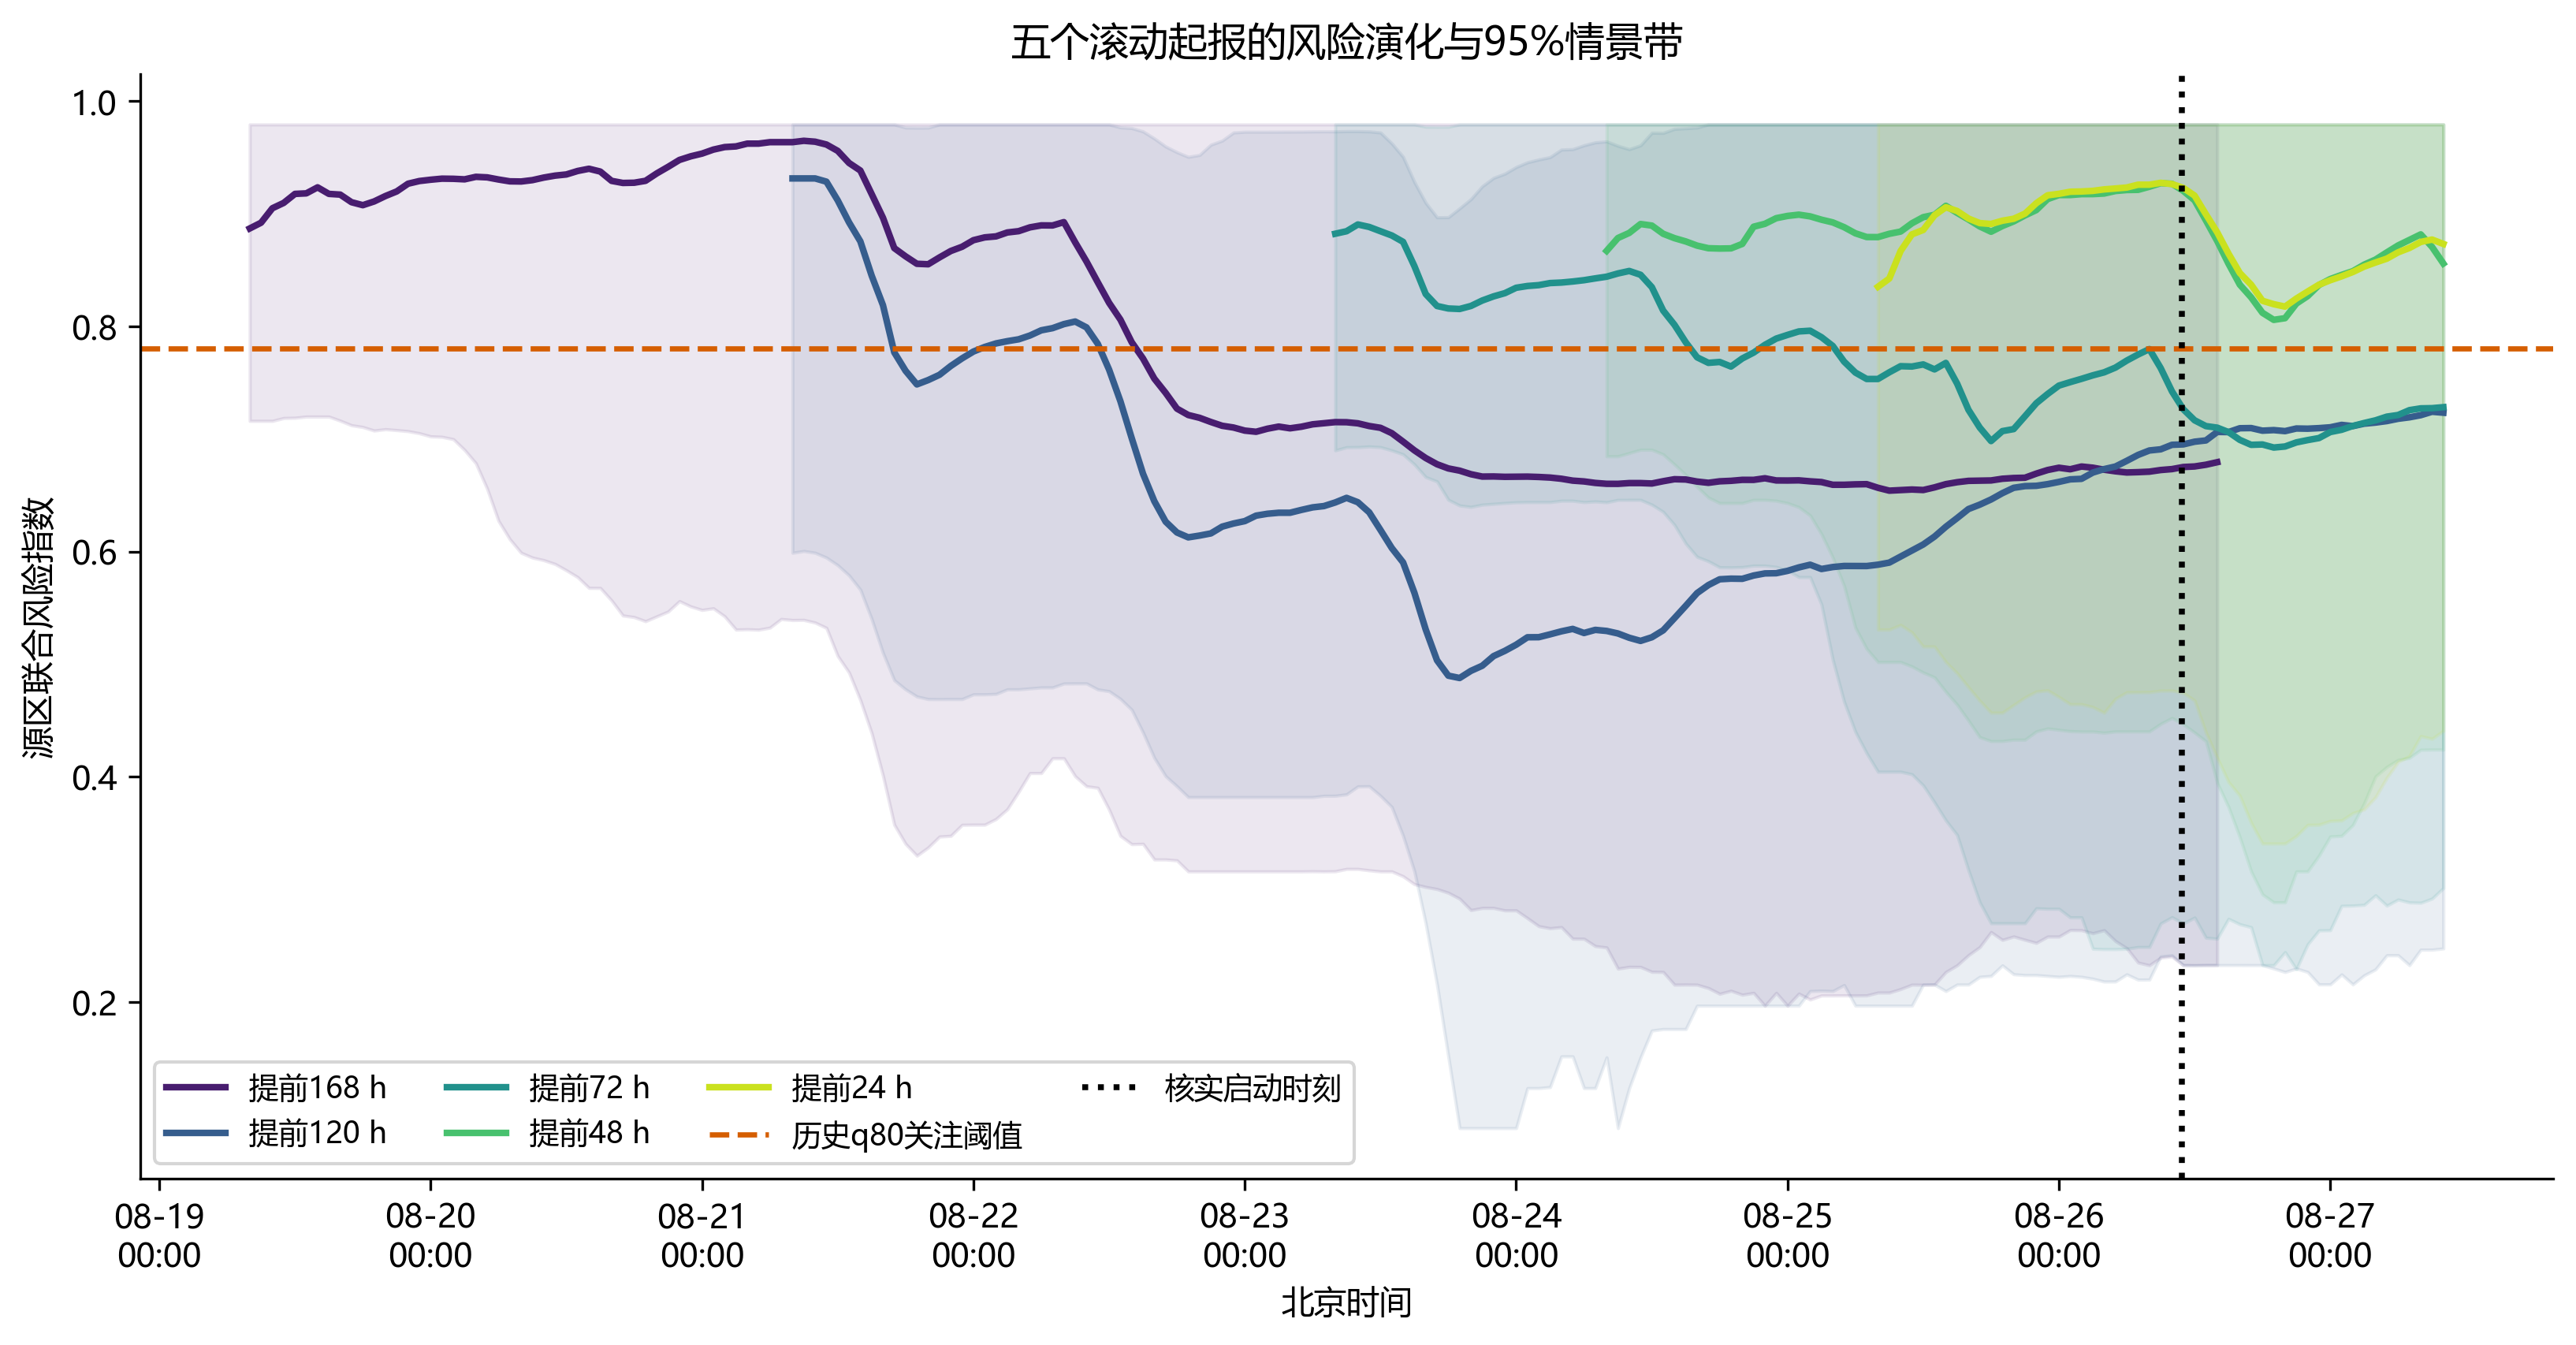
\includegraphics[width=\linewidth]{figures/q3/q3_fig01.png}
 \caption{五次滚动起报的联合风险演化与95\%情景带}
 \label{fig:q3-risk}
\end{figure}

对每条情景序列求取触发时刻，汇总得到表\ref{tab:q3-results}，时间区间见图\ref{fig:q3-time}。表中日期均为2026年8月，点误差以核实启动时刻为基准计算。
\begin{table}[htbp]
 \centering
 \zihao{-5}
 \caption{五起报确定性基线与集合模型求解结果}
 \label{tab:q3-results}
 \setlength{\tabcolsep}{3.5pt}
 \begin{tabularx}{\textwidth}{c c c c c X}
 \toprule
 名义/实际 & 基线时刻 & 集合中位时刻 & 集合误差 & 支持比例 & 原始95\%情景区间\\
 提前量/h & （误差/h） & （月-日 时:分） & /h & /\% & （月-日 时:分）\\
 \midrule
 168/170.87 & 21日11:00 (119.87) & 08-20 20:00 & 134.87 & 85.0 & 08-19 19:00至08-26 06:00\\
 120/122.87 & 21日19:00 (111.87) & 08-21 19:00 & 111.87 & 69.5 & 08-21 19:00至08-27 10:00\\
 72/74.87 & 23日19:00 (63.87) & 08-24 12:00 & 46.87 & 70.6 & 08-23 19:00至08-27 10:00\\
 48/50.87 & 26日10:00 (0.87) & 08-26 08:00 & 2.87 & 73.7 & 08-24 19:00至08-27 10:00\\
 24/26.87 & 26日10:00 (0.87) & 08-26 11:00 & 0.13 & 74.4 & 08-25 19:00至08-27 10:00\\
 \bottomrule
 \end{tabularx}
\end{table}
\begin{figure}[htbp]
 \centering
 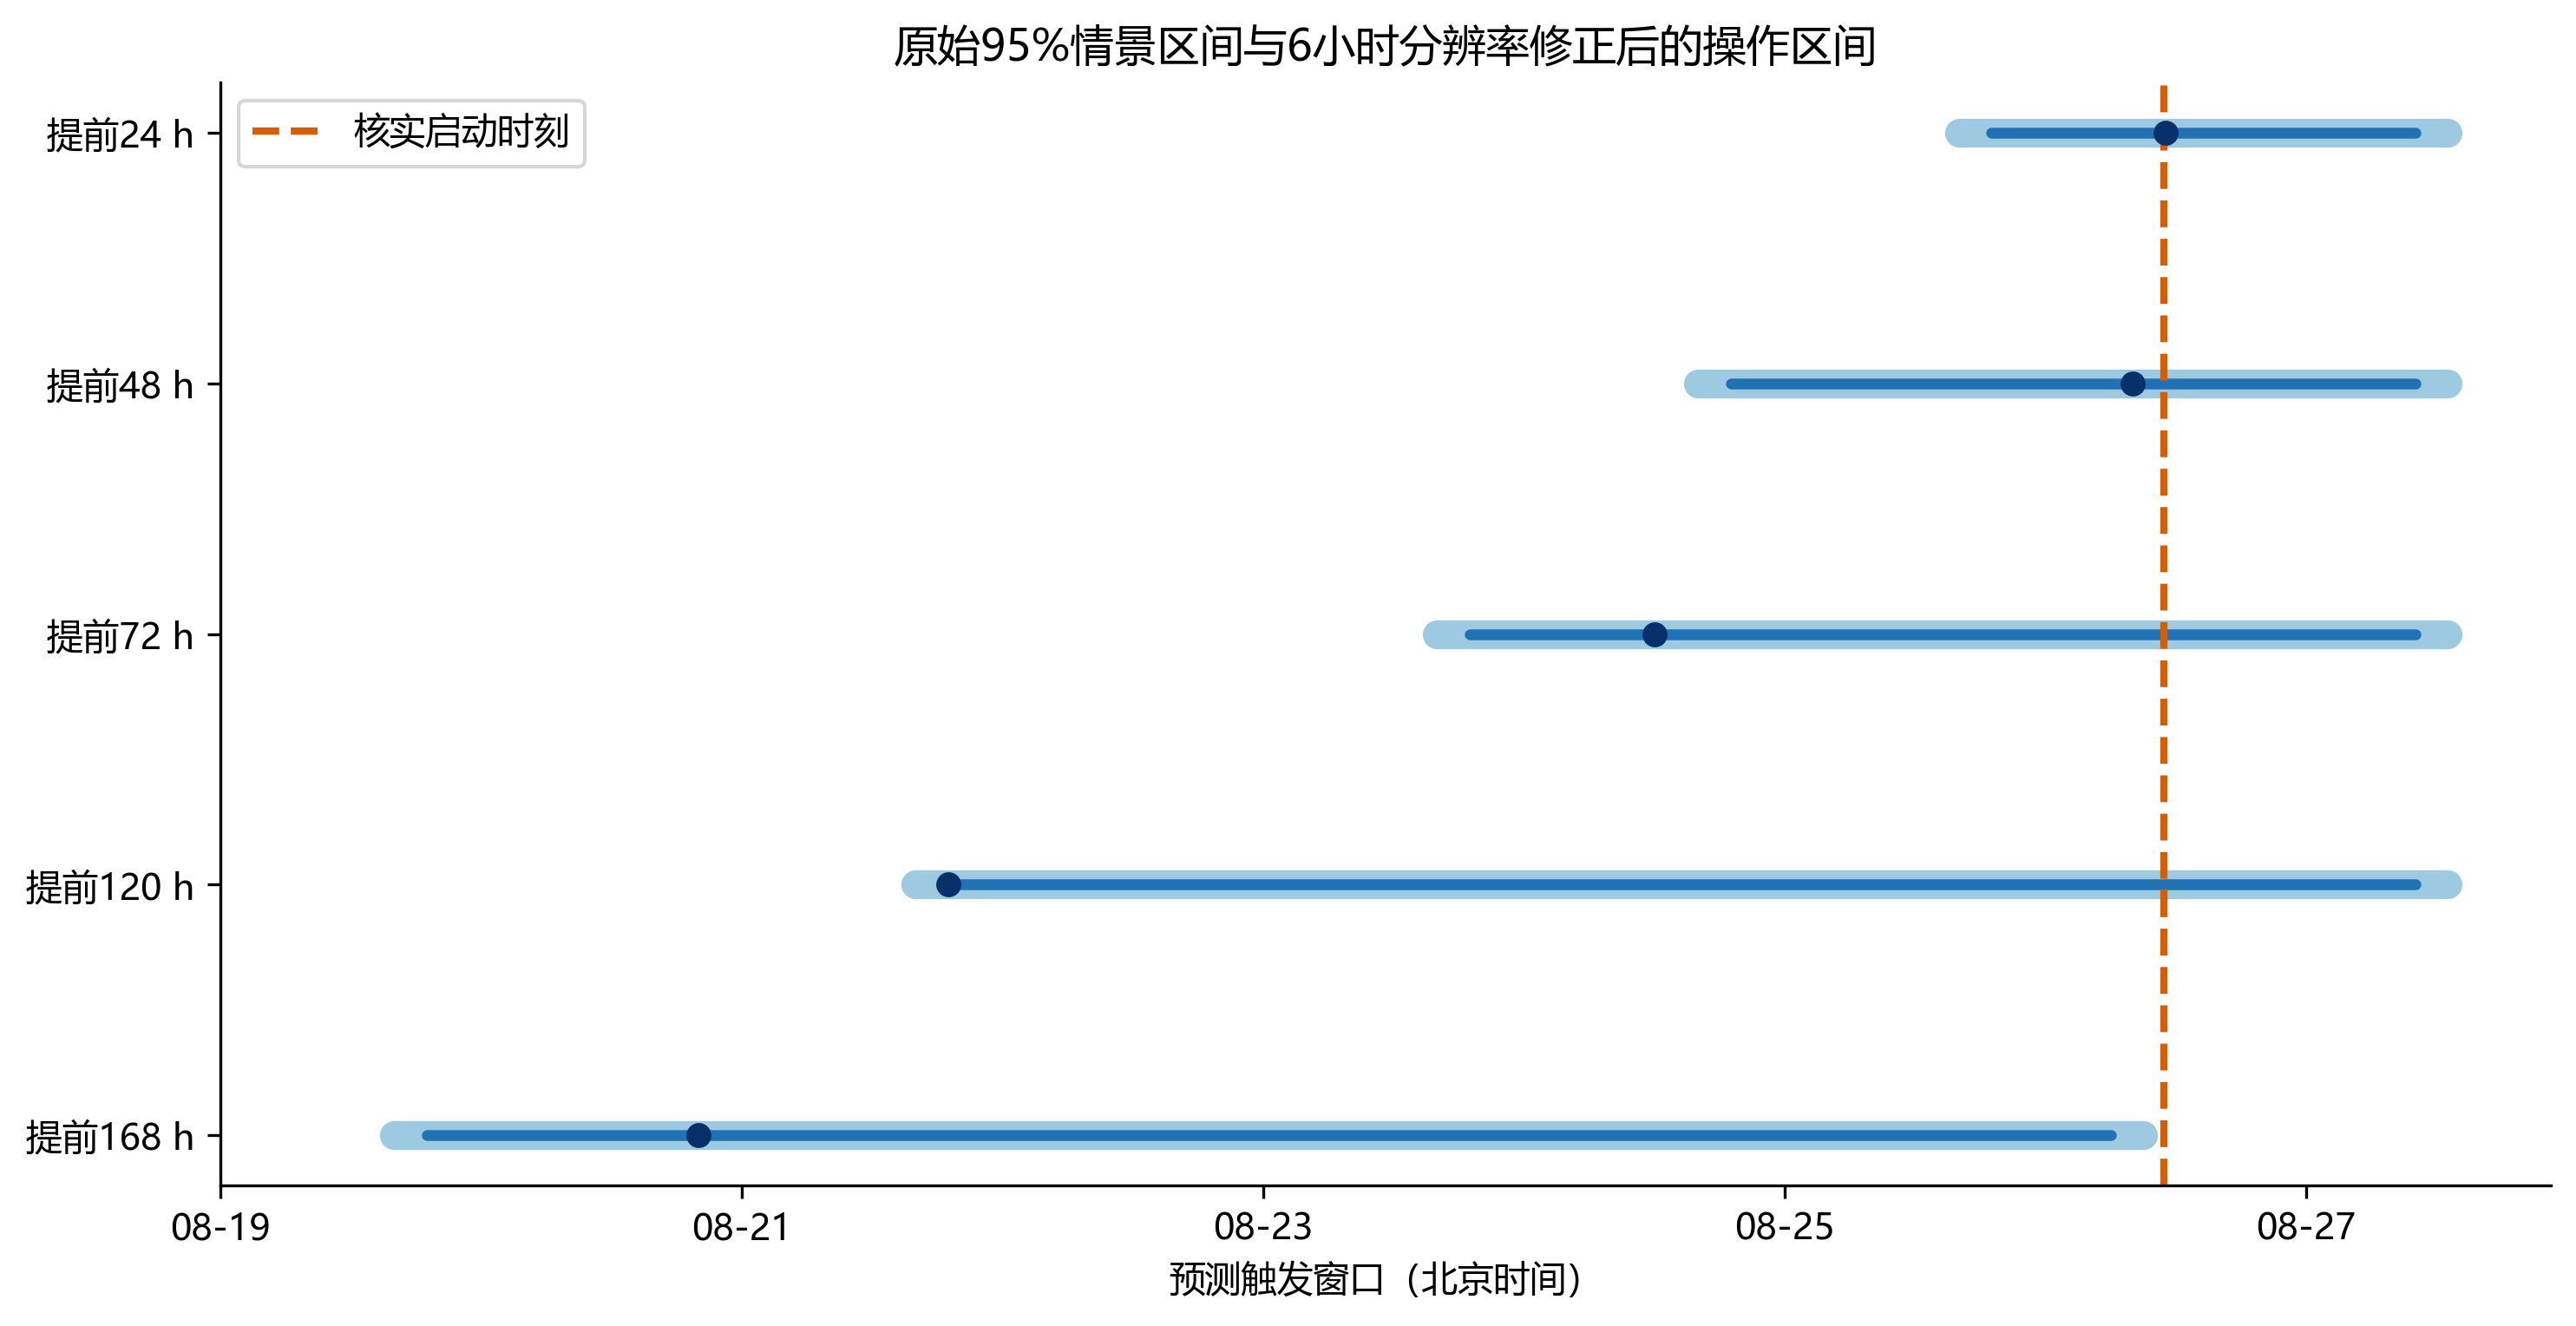
\includegraphics[width=\linewidth]{figures/q3/q3_fig02.png}
 \caption{五次起报的触发时间中位数、原始情景区间与操作区间}
 \label{fig:q3-time}
\end{figure}

表\ref{tab:q3-results}中，24 h起报的中位触发时刻为8月26日11:00，较核实启动晚0.13 h；48 h起报为当日08:00，提前2.87 h。两次中位时刻均定位在事件日，对应原始区间宽39 h和63 h，操作区间宽45 h和69 h。点估计接近核实时刻时，情景分布仍跨越数十小时，预警时需同时考虑危险窗口的宽度。

随起报临近事件，原始区间宽度由155 h依次缩小为135、87、63和39 h，表明危险窗口逐步收窄。168 h区间上界早于实际启动。与确定性基线相比，集合中位时刻的误差在24 h和72 h起报中减小，120 h相同，48 h和168 h增大。集合模型的作用主要是给出风险分散程度及其随提前量的变化，点估计的改善则因起报而异。

按核实启动时刻$t_*$是否落入第$i$次起报区间$\mathcal I_i$，计算描述性覆盖比例$\widehat C=\frac{1}{5}\sum_{i=1}^{5}\mathbf1\{t_*\in\mathcal I_i\}$。本事件五次滚动回放中，两类区间均覆盖4次，比例为80\%。

\subsubsection{预警时间与主导机制分析}
图\ref{fig:q3-warning}给出了五次起报的预警等级和机制诊断。168 h起报达到持续红色，120 h回落至常态，72 h为蓝色，48 h与24 h均达到橙色，后两次起报的等级判断一致。48 h起报预测橙色持续过程从8月25日20:00开始，提前14.87 h；24 h起报预测从当日13:00开始，提前21.87 h。两次起报均从各自08:00起报时进入蓝色关注状态，对应实际起报提前量50.87 h和26.87 h。上述过程起点均根据起报所预测的后续12 h风险确定。
\begin{figure}[htbp]
 \centering
 \begin{subfigure}{\linewidth}
   \centering
   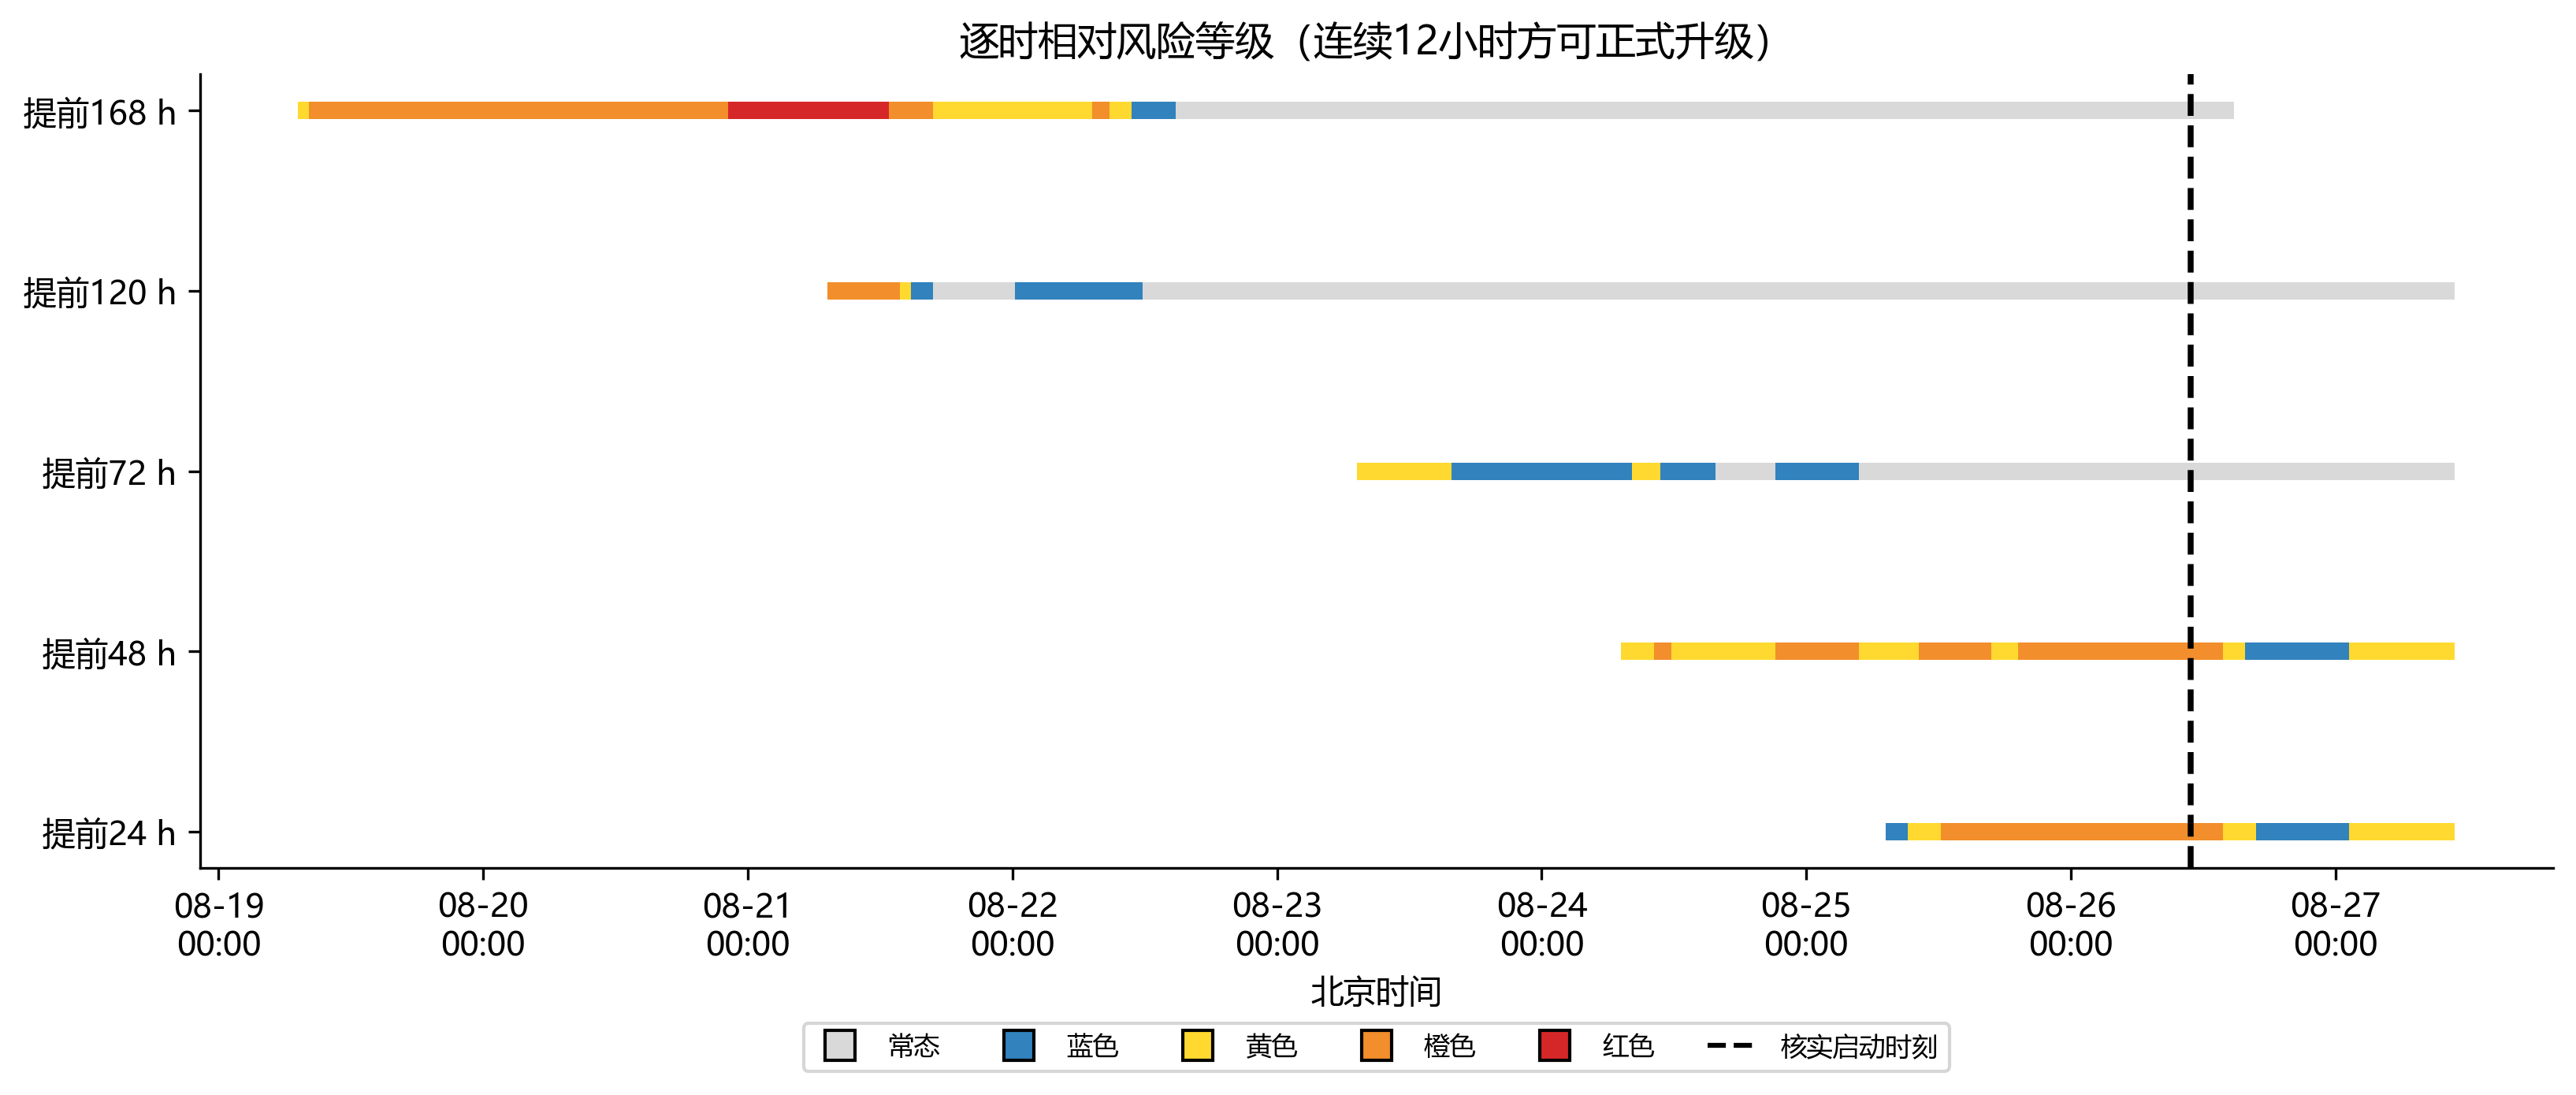
\includegraphics[width=0.88\linewidth]{figures/q3/q3_fig06.png}
   \caption{滚动预警等级时间轴}
 \end{subfigure}
 \par\medskip
 \begin{subfigure}{\linewidth}
   \centering
   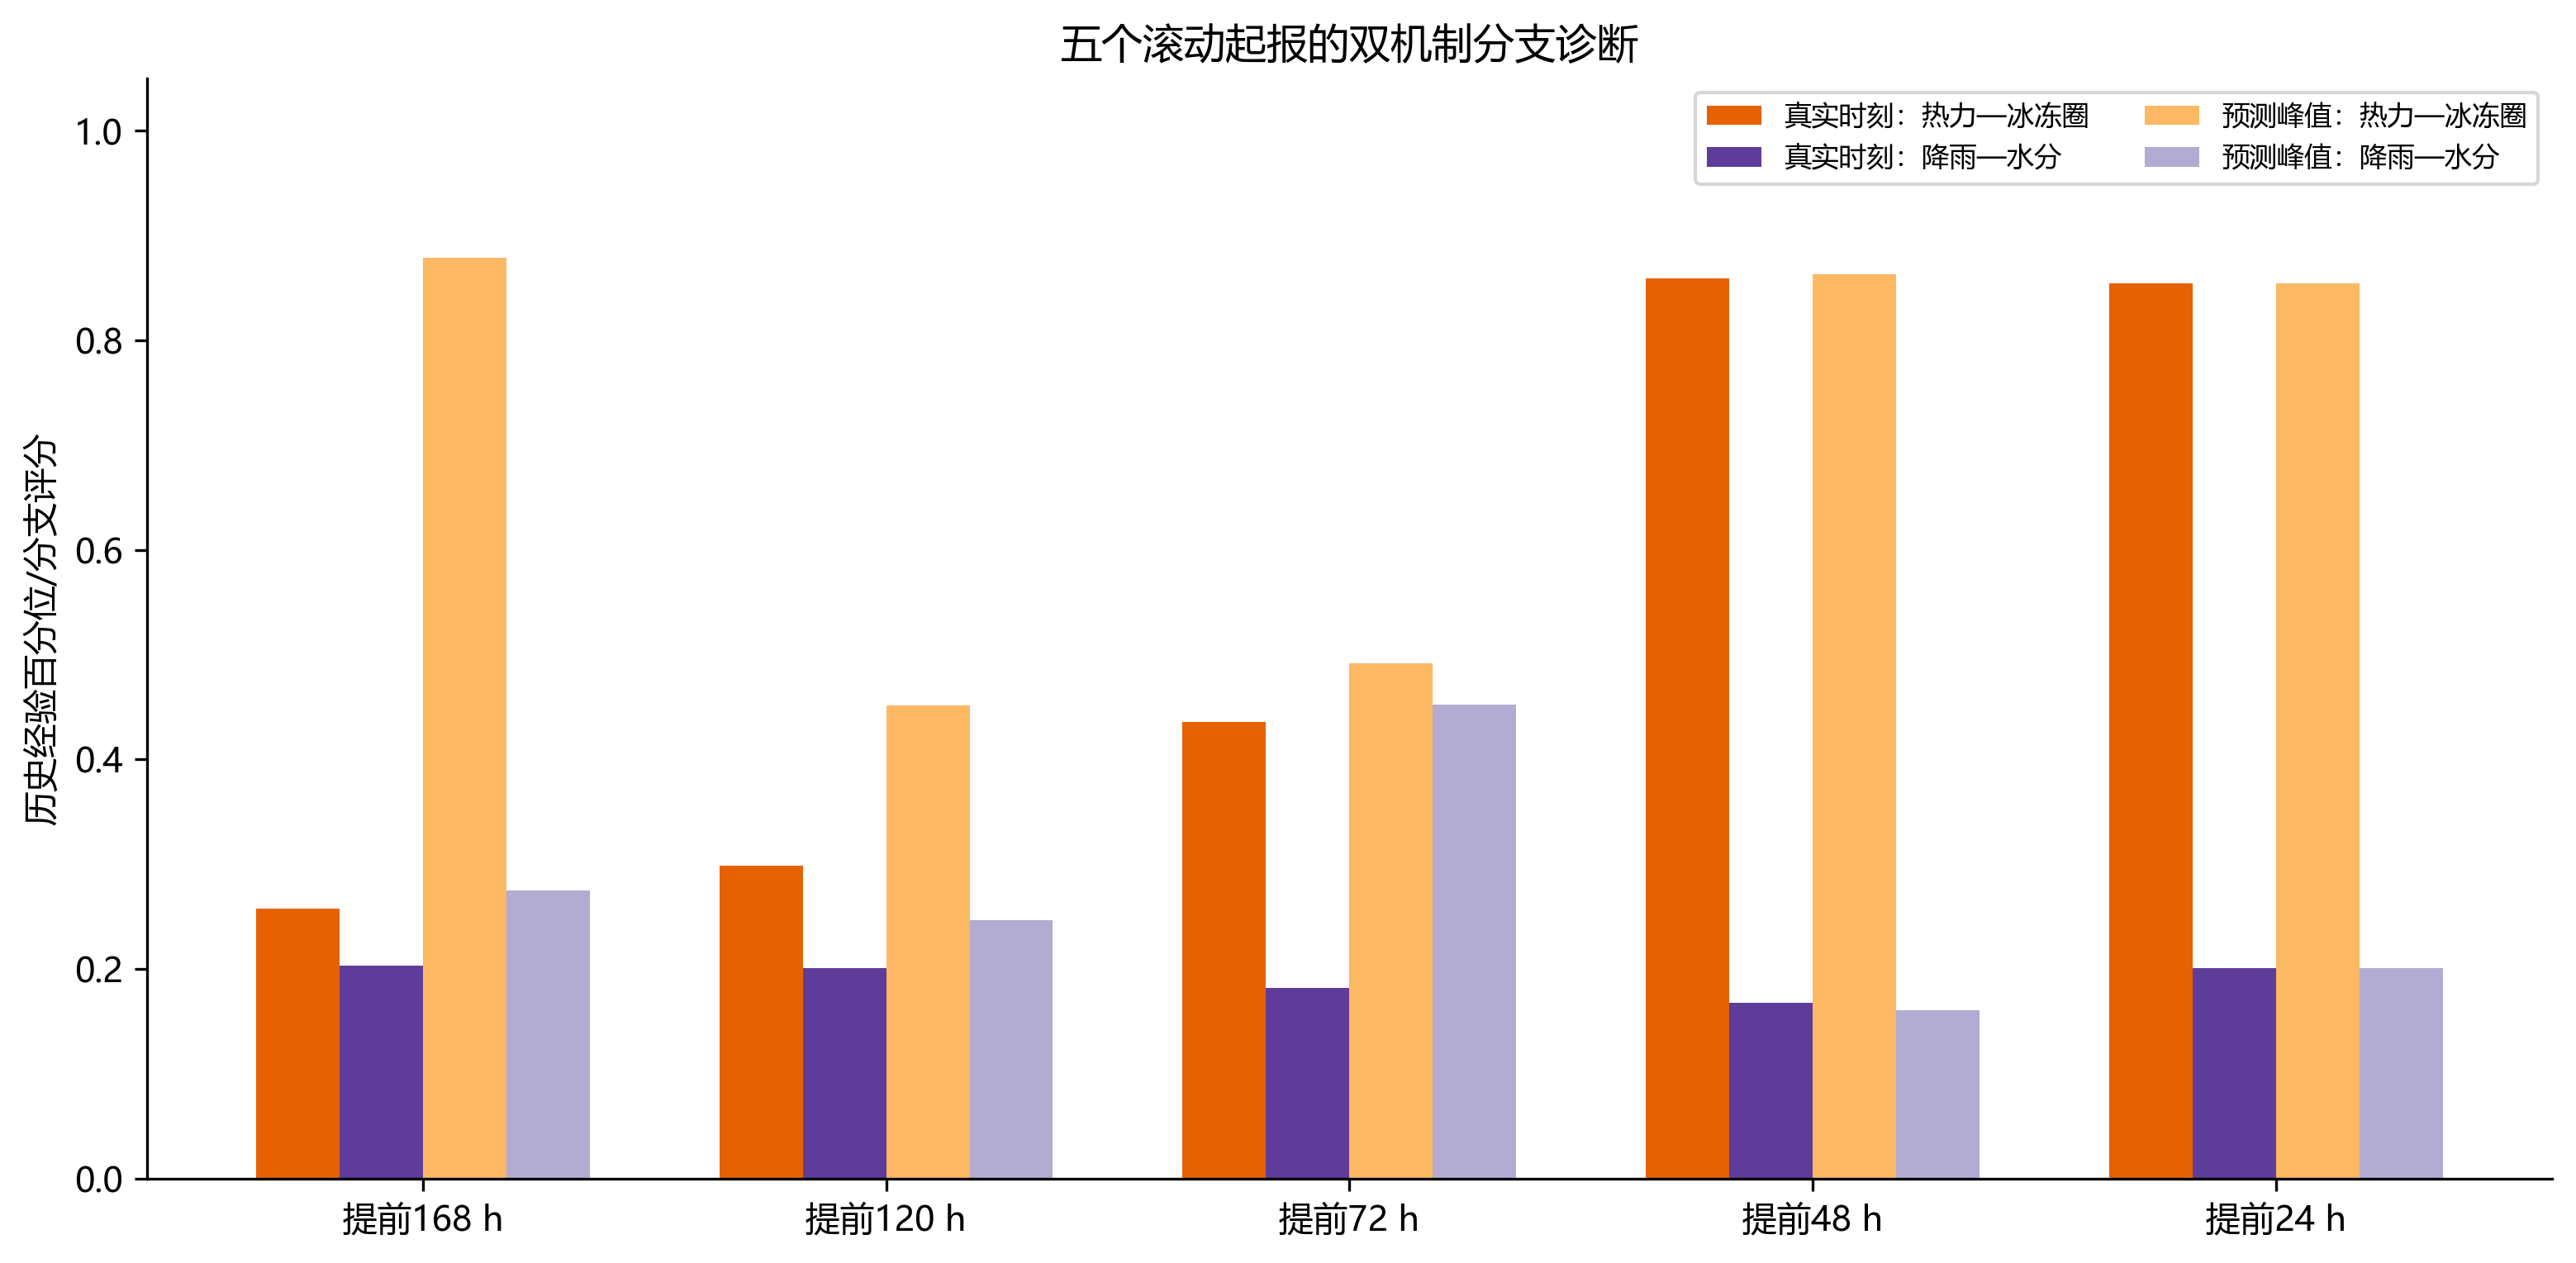
\includegraphics[width=0.88\linewidth]{figures/q3/q3_fig07.png}
   \caption{热力—冰冻圈与降雨—水分分支诊断}
 \end{subfigure}
 \caption{五次起报的相对预警等级与双机制结果}
 \label{fig:q3-warning}
\end{figure}

在距核实启动最近的11:00时次，五次起报的热力分支得分均高于降雨—水分分支。48 h起报的热力与降雨—水分得分分别为0.859和0.168，24 h为0.855和0.201。这与第一问识别的暖、干及能量偏强背景一致。

IMERG用于独立核验起报前的降雨。按Late Run的14 h名义延迟\footnote{NASA GPM：\url{https://gpm.nasa.gov/resources/faq/what-determines-latency-imerg}。}截断，仅使用$t_i-14\ \mathrm{h}$及以前结束的资料，核验窗完整度至少为95\%。计算结果表明，48 h与24 h起报的完整72 h累计量为5.86 mm和6.40 mm，均低于历史$q_{0.90}=39.83$ mm；按启动时刻回溯的72 h累计量为8.33 mm。168、120与72 h起报的资料窗不完整，记为不可判。完整窗口中的降雨水平支持本事件以热力分支为主的解释。

\subsubsection{口岸到达时间与沿程传播距离}
将有效触发时刻与分段速度情景结合，得到图\ref{fig:q3-propagation}。源区至口岸的水平中心线长20.909 km，地形修正长度为21.681 km。五次起报的传播时间中位数均在7.38—7.39 min之间；以24 h起报为例，中位数为7.39 min，95\%范围为7.12—7.70 min。各次计算使用相同路径，差别来自情景抽样。
\begin{figure}[htbp]
 \centering
 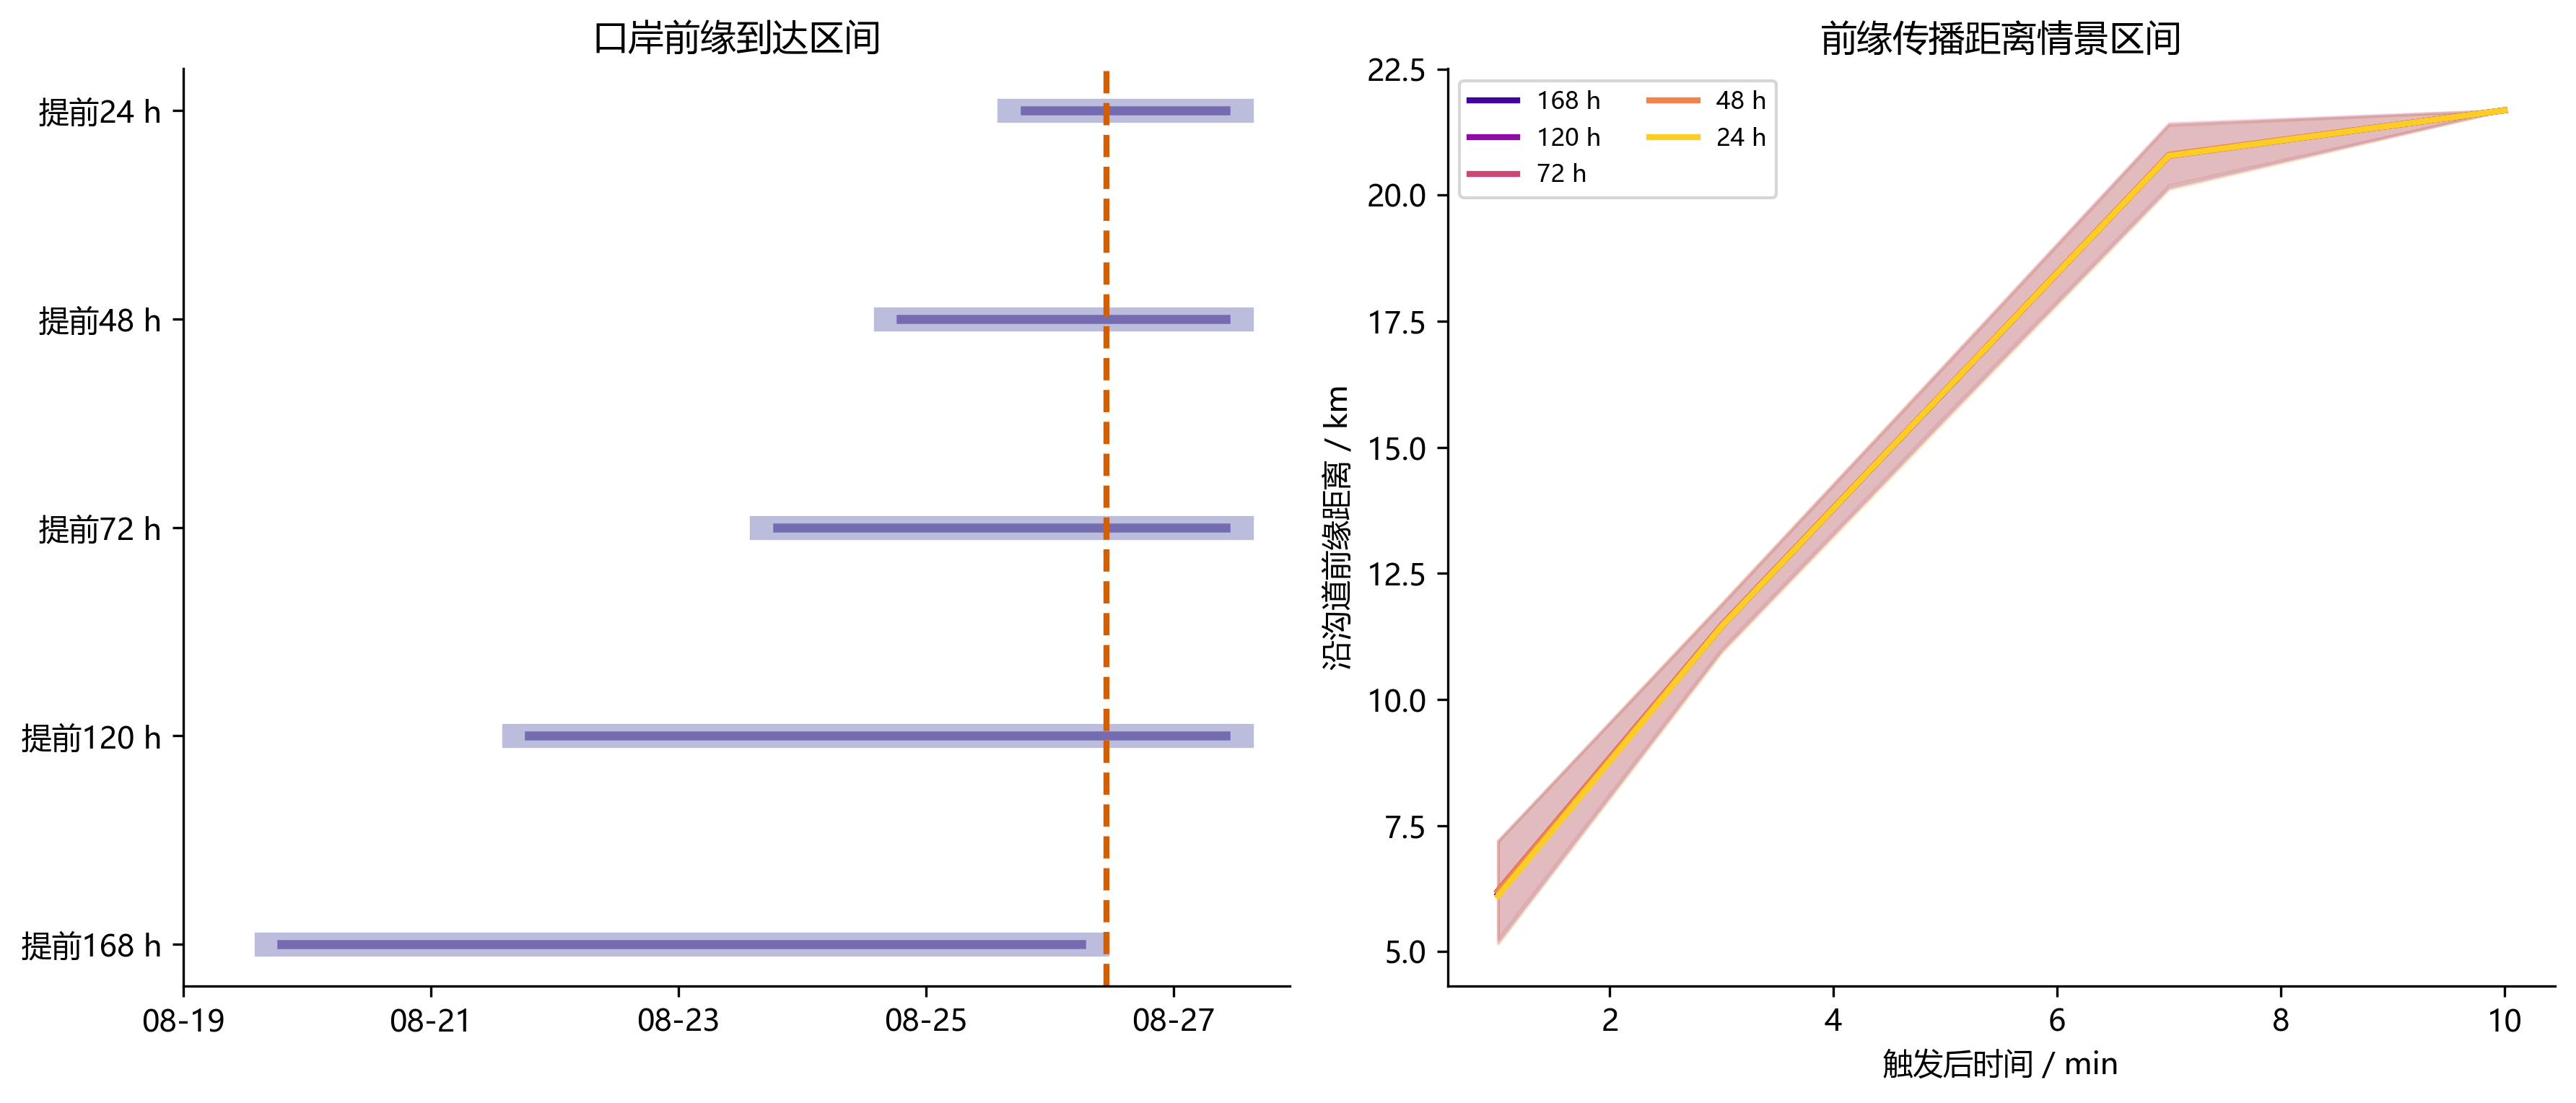
\includegraphics[width=\linewidth]{figures/q3/q3_fig04.png}
 \caption{口岸到达时间区间及触发后沿程前缘距离}
 \label{fig:q3-propagation}
\end{figure}

24 h起报预测口岸到达中位时刻为8月26日11:07，原始区间为8月25日19:07至27日10:07，操作区间向两端各扩展3 h；48 h起报的中位时刻为8月26日08:07。触发时刻的分散程度为小时量级，传播时间的波动为分钟量级，因而口岸到达区间主要取决于源区触发区间。

24 h起报的前缘在触发后1、3、5和7 min分别推进至6.10、11.45、16.12和20.78 km，以上均为情景中位数。10 min时各情景已到达D点，计算距离固定为21.681 km，对应源区至口岸的既定路径长度。D点之后的传播及二维影响范围、泥深、流速场和承灾体暴露，由第四问动力学模型进一步计算。

\subsubsection{窗口敏感性与结果的适用范围}
保持主方案72/72/120 h混合窗口，另将融水、降水和根区水分统一设为24、48、72、120、168 h进行检验。以五次起报中位时刻绝对误差的中位数衡量，主方案为46.87 h，统一24、48 h窗口分别为26.87、25.87 h，统一120、168 h窗口均为63.87 h。各方案原始区间覆盖4次；统一24、48 h方案的操作区间覆盖5次。

短窗口在本次回放中的误差较低，说明累积尺度会影响风险峰值的定位。主模型采用第二问预先确定的混合窗口，上述结果用于考察窗口敏感性。

历史源区热点超过$q_{0.80}$的比例为79.8\%，蓝色等级用于持续关注；$J_t$、情景支持比例及四色等级均按相对风险解释，发生概率和虚警率需用独立事件标定。

本问结果来自已知事件评价窗和灾后反演速度下的回放，遥感缓存、缺测插补及产品发布时间仍需逐起报冻结核验。就本次事件而言，24—48 h起报可用于定位危险窗口，72 h及以上起报用于形势研判；跨事件检验还需长期预报档案和源区监测。



\end{document}
